\documentclass{article}
\usepackage[utf8]{inputenc}
\usepackage[ngerman]{babel}

% Convenience improvements
\usepackage{csquotes}
\usepackage{enumitem}
\setlist[enumerate,1]{label={\alph*)}}
\usepackage{amsmath}
\usepackage{amssymb}
\usepackage{mathtools}
\usepackage{tabularx}
\usepackage{listings}

% Proper tables and centering for overfull ones
\usepackage{booktabs}
\usepackage{adjustbox}

% Change page/text dimensions, the package defaults work fine
\usepackage{geometry}

\usepackage{parskip}

% Drawings
\usepackage{tikz}
\usepackage{pgfplots}

% Adjust header and footer
\usepackage{fancyhdr}
\pagestyle{fancy}
\fancyhead[L]{Computernetzwerke --- \textbf{Übung 8}}
\fancyhead[R]{Laurenz Weixlbaumer (11804751)}
\fancyfoot[C]{}
\fancyfoot[R]{\thepage}
% Stop fancyhdr complaints
\setlength{\headheight}{12.5pt}

\newcommand{\Deltaop}{\, \Delta\, }
\newcommand{\xor}{\, \oplus\, }
\newcommand{\id}{\text{id}}

\begin{document}

\paragraph{Aufgabe 1.}

\begin{enumerate}
    \item[(a) und (b)] Router arbeiten auf Schicht 3, sehen also die Zieladresse. Nach Erhalt eines Pakets durchsucht der Router seine Routing-Tabelle nach der Zieladresse und leitet das Paket an jene Adresse weiter, die der Zieladresse am besten entspricht. Spezifischere Adressen bzw. Matches werden vor weniger spezifischen gewählt. Kann so keine Adresse gefunden werden wird das Paket an das Standardgateway weitergeleitet.
    
    \item[(c)] RIP, EIGRP, OSPF und IS-IS sind \emph{Interiour Gateway} Protokolle, die innerhalb eines \enquote{autonomen Systems} (eine administrative Struktur, z.B. innerhalb einer Firma) verwendet werden. Als solche sind sie auf Geschwindigkeit und Reaktivität ausgelegt. Weiters wird zwischen \emph{Distance Vector} (RIP und EIGRP) und \emph{Link State} (DSPF, IS-IS) Protokollen unterschieden. Erstere kennen nur ihre nächsten Nachbarn (nur Next-Hop), brauchen somit vergleichsweise wenig Rechenkraft und Speicherplatz, sind aber weniger Fehlerresistent. Letztere kennen die gesamte Netzwerktopologie, sind somit Ressourcenhungriger, können aber im Fehlerfall sofort Alternativrouten finden.

    BGP ist ein \emph{Exteriour Gateway} Protokoll, verwendet für Kommunikation zwischen autonomen Systemen (etwa Firma --- ISP). Als solches ist es primär auf Stabilität ausgelegt und bietet zudem mehr Sicherheitsfeatures --- etwa Schutzmaßnahmen vor bösartigen Nachahmungen von Netzen durch Schadakteure.
\end{enumerate}

\paragraph{Aufgabe 2.}

\begin{enumerate}
    \item Screenshots der PCs:

    \begin{center}
        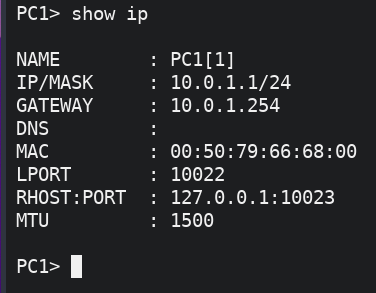
\includegraphics[width=.3\textwidth]{img/pc1.png}
        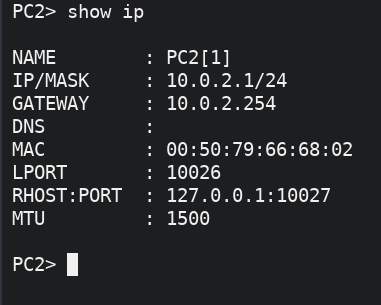
\includegraphics[width=.3\textwidth]{img/pc2.png}
        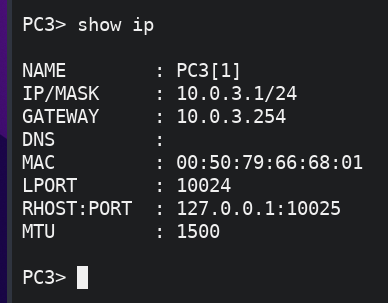
\includegraphics[width=.3\textwidth]{img/pc3.png}
    \end{center}

    Screenshots der Router (in Reihenfolge ISP, 1, \ldots, 5):

    \begin{center}
        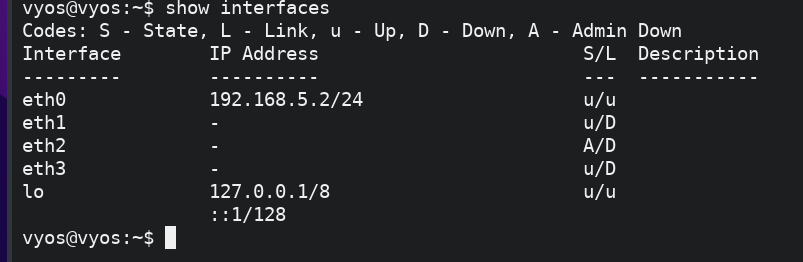
\includegraphics[width=.45\textwidth]{img/r-isp.png}
        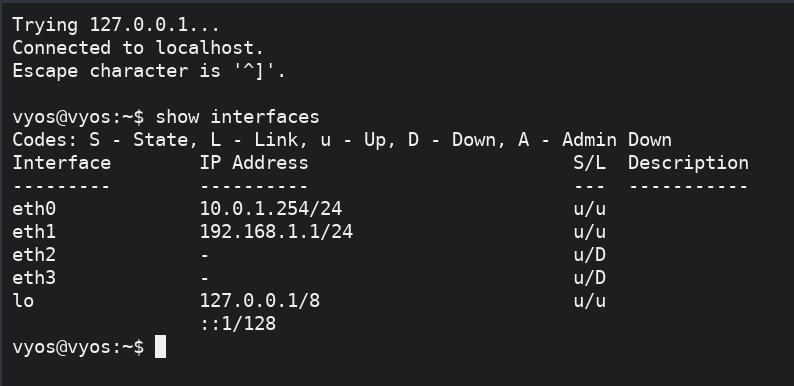
\includegraphics[width=.45\textwidth]{img/r1.png}
        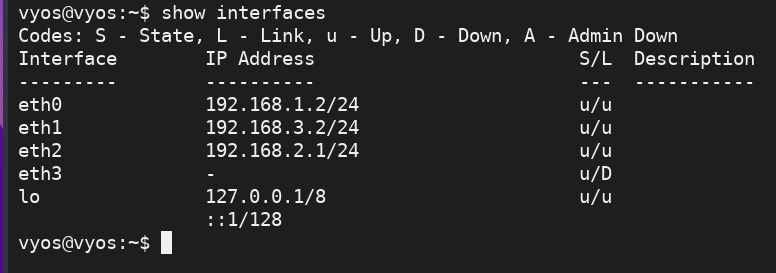
\includegraphics[width=.45\textwidth]{img/r2.png}
        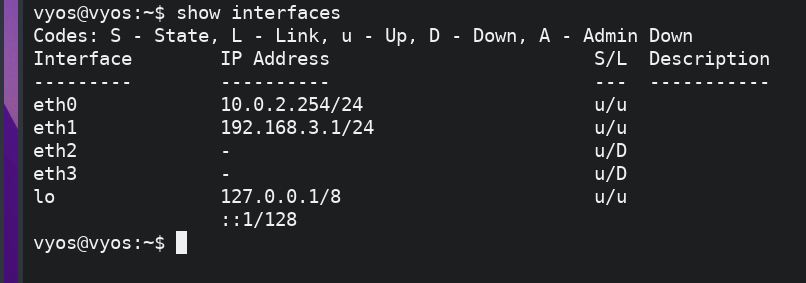
\includegraphics[width=.45\textwidth]{img/r3.png}
        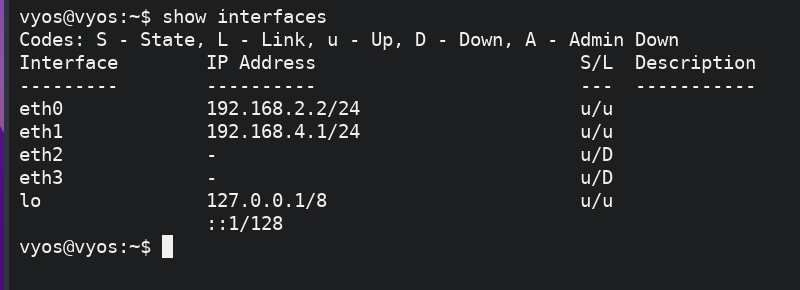
\includegraphics[width=.45\textwidth]{img/r4.png}
        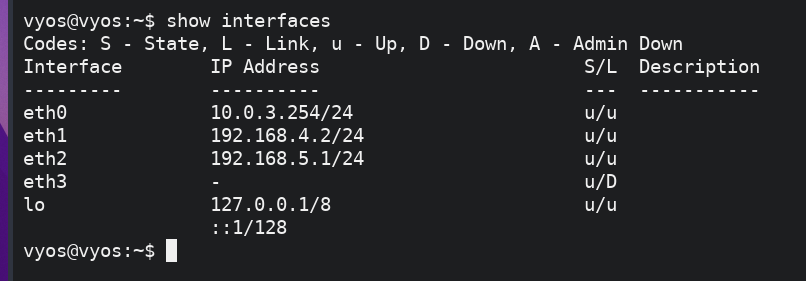
\includegraphics[width=.45\textwidth]{img/r5.png}
    \end{center}

    Screenshot der Topologie:

    \begin{center}
        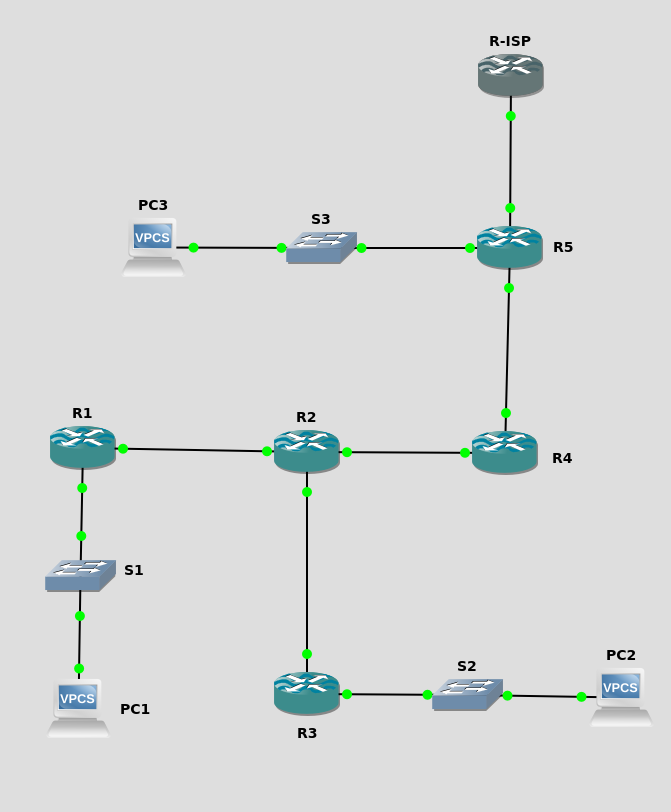
\includegraphics[width=.5\textwidth]{img/topology.png}
    \end{center}

    \item Die Konfiguration der default gateways der PC ist aus den obigen Screenshots ersichtlich. Screenshots der Router (in Reihenfolge 1 bis 5):
    
    \begin{center}
        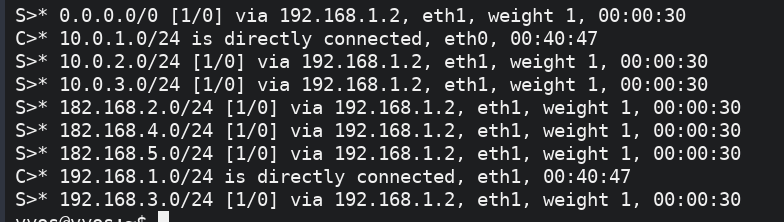
\includegraphics[width=.45\textwidth]{img/rr1.png}
        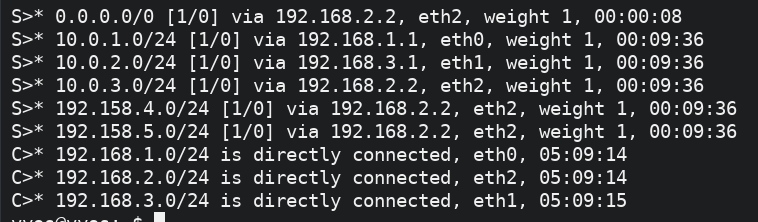
\includegraphics[width=.45\textwidth]{img/rr2.png}
        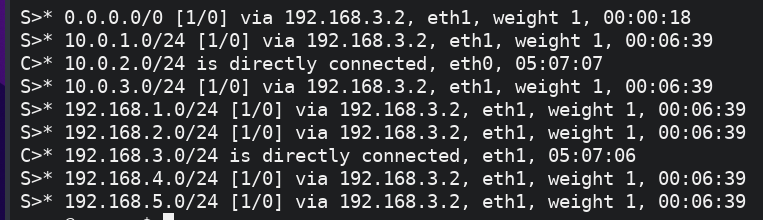
\includegraphics[width=.45\textwidth]{img/rr3.png}
        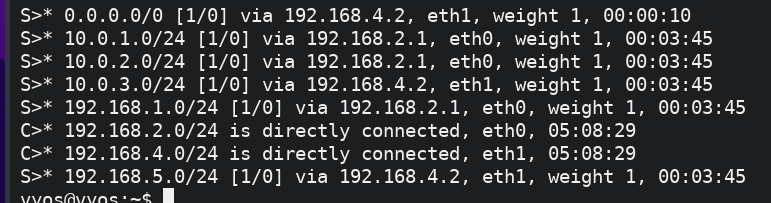
\includegraphics[width=.45\textwidth]{img/rr4.png}
        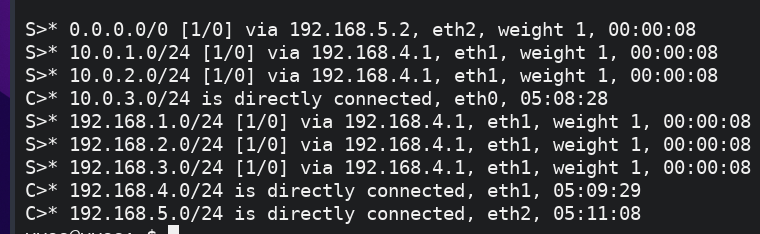
\includegraphics[width=.45\textwidth]{img/rr5.png}
    \end{center}

    Ping und trace zur Verifikation:

    \begin{center}
        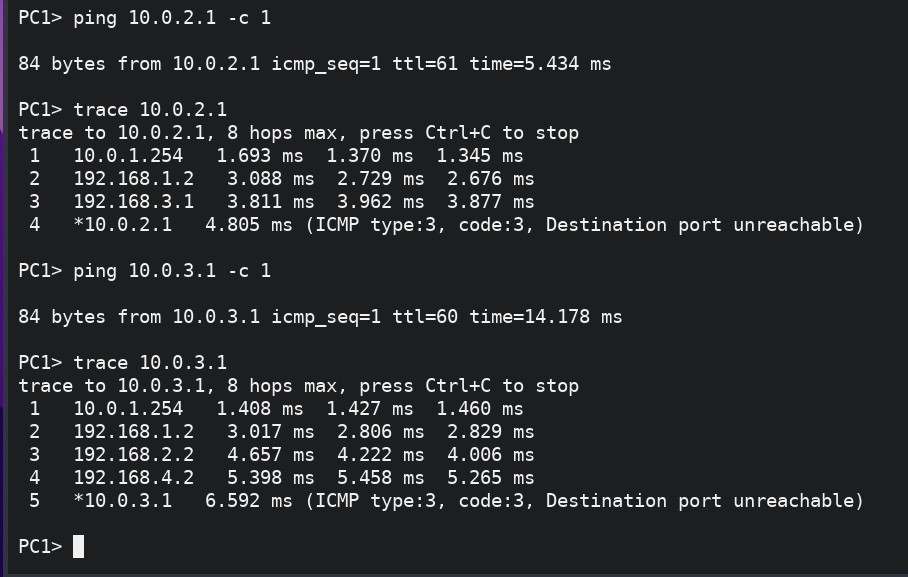
\includegraphics[width=.45\textwidth]{img/pt1.png}
        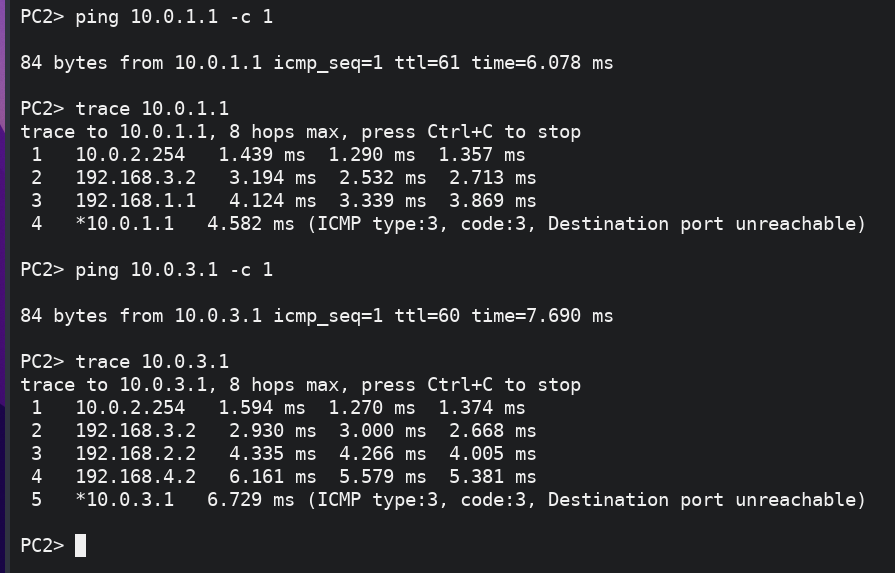
\includegraphics[width=.45\textwidth]{img/pt2.png}
        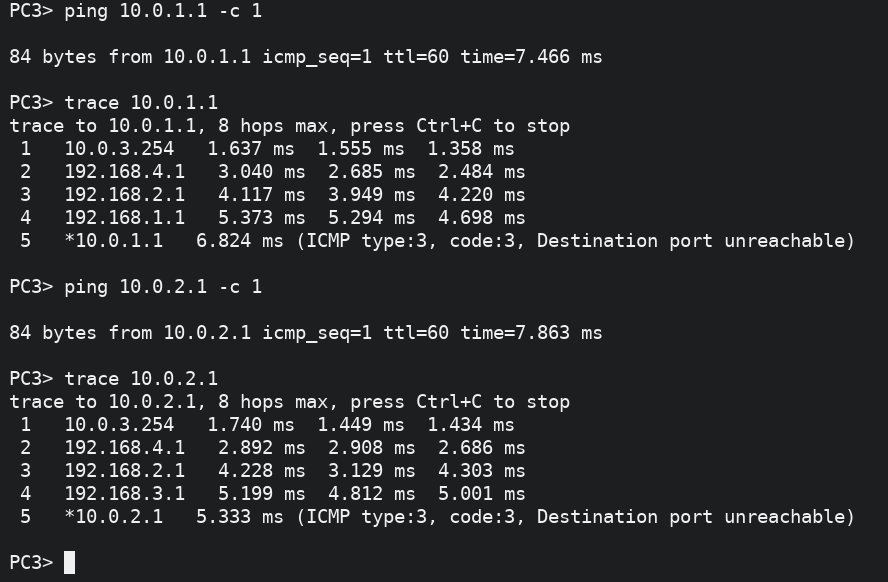
\includegraphics[width=.45\textwidth]{img/pt3.png}
    \end{center}

    \item Routen lassen sich aggregieren, wenn ihr next-hop gleich ist und die Zielnetzaddressen zusammengefasst werden können. So könnten in R1 etwa die Routen für 10.0.2.0/24 und 10.0.3.0/24 auf 10.0.2.0/23 zusammengefasst werden. (Tatsächlich könnten in R1 sogar alle Routen bis auf die Defaultroute weggelassen werden, alle Wege führen nach R2.)
\end{enumerate}

\end{document}
